% tugas_data_analitik.tex
% Laporan Tugas Data Analitik — C-MAPSS RUL Prediction
% Departemen Teknik Mesin FTUI — 2026

\documentclass[11pt,a4paper]{article}

% ── Packages ──────────────────────────────────────────────────────────────────
\usepackage[T1]{fontenc}
\usepackage[utf8]{inputenc}
\usepackage[a4paper, margin=2.5cm]{geometry}
\usepackage{setspace}
\usepackage{parskip}
\usepackage{titlesec}
\usepackage{fancyhdr}
\usepackage{booktabs}
\usepackage{tabularx}
\usepackage{multirow}
\usepackage{longtable}
\usepackage{graphicx}
\usepackage{caption}
\usepackage{subcaption}
\usepackage{xcolor}
\usepackage{amsmath}
\usepackage{hyperref}
\usepackage{enumitem}
\usepackage{float}
\usepackage{tocloft}
\usepackage{amssymb}

% ── Colors ────────────────────────────────────────────────────────────────────
\definecolor{uiblue}{RGB}{0,56,147}
\definecolor{mygray}{RGB}{100,100,100}

% ── Section formatting ────────────────────────────────────────────────────────
\titleformat{\section}
  {\large\bfseries\color{uiblue}}
  {\thesection}{0.6em}{}[\vspace{2pt}\hrule\vspace{4pt}]

\titleformat{\subsection}
  {\normalsize\bfseries\color{uiblue}}
  {\thesubsection}{0.6em}{}

\titleformat{\subsubsection}
  {\small\bfseries}
  {\thesubsubsection}{0.6em}{}

% ── Header / Footer ───────────────────────────────────────────────────────────
\pagestyle{fancy}
\fancyhf{}
\fancyhead[L]{\small\color{mygray}
  Tugas Data Analitik -- Prediksi RUL Mesin Turbofan C-MAPSS}
\fancyhead[R]{\small\color{mygray} Departemen Teknik Mesin FTUI}
\fancyfoot[C]{\small\color{mygray}\thepage}
\renewcommand{\headrulewidth}{0.4pt}
\renewcommand{\footrulewidth}{0.0pt}

\onehalfspacing
\captionsetup{font=small, labelfont=bf}

\hypersetup{
  colorlinks=true,
  linkcolor=uiblue,
  urlcolor=uiblue,
  citecolor=uiblue,
}

% ══════════════════════════════════════════════════════════════════════════════
\begin{document}

% ── Cover Page ────────────────────────────────────────────────────────────────
\begin{titlepage}
  \centering
  \vspace*{1.0cm}

  
\includegraphics[width=2.2cm]{images/logo_ui.png}

  \vspace{0.6cm}
  {\large\bfseries UNIVERSITAS INDONESIA\par}
  \vspace{0.2cm}
  {\normalsize Fakultas Teknik -- Departemen Teknik Mesin\par}

  \vspace{0.5cm}
  \hrule height 1.2pt
  \vspace{0.4cm}
  {\LARGE\bfseries\color{uiblue}
    PREDIKSI \textit{REMAINING USEFUL LIFE}\\[0.3em]
    MESIN TURBOFAN MENGGUNAKAN\\[0.3em]
    \textit{ARTIFICIAL NEURAL NETWORK}\\[0.3em]
    PADA DATASET C-MAPSS\par}
  \vspace{0.4cm}
  \hrule height 1.2pt

  \vspace{1.0cm}
  {\normalsize\color{mygray} Mata Kuliah:\par}
  {\large\bfseries Data Analitik\par}

  \vspace{0.6cm}
  {\normalsize\color{mygray} Dosen Pengampu:\par}
  {\normalsize Dr.\ Eng.\ Sholahudin, S.T., M.Sc.\par}

  \vspace{0.8cm}
  {\normalsize\color{mygray} Disusun Oleh:\par}
  \vspace{0.4cm}
  \begin{tabular}{ll}
    2506565466 & Luqman Alifio Arhab \\[4pt]
    2506565414 & Azfa Rhazasta Abiandra \\[4pt]
    2506565401 & Adamsyah Haryo Saksono \\[4pt]
    2506565433 & Epsiarto Rizqi Nurwijayadi \\[4pt]
  \end{tabular}

  \vspace{0.2cm}
  \vfill
  {\normalsize\bfseries
    DEPARTEMEN TEKNIK MESIN\\
    FAKULTAS TEKNIK\\
    UNIVERSITAS INDONESIA\\[0.4em]
    2026\par}
\end{titlepage}

\thispagestyle{empty}
\newpage
\setcounter{page}{1}

% ── Table of Contents ─────────────────────────────────────────────────────────
\tableofcontents
\newpage

% ══════════════════════════════════════════════════════════════════════════════
\section{Pendahuluan}

\subsection{Latar Belakang}

Prediksi \textit{Remaining Useful Life} (RUL) merupakan komponen kunci dalam
sistem \textit{Prognostics and Health Management} (PHM) peralatan mekanik.
Dengan mengetahui sisa umur pakai suatu komponen sebelum kegagalan terjadi,
jadwal perawatan dapat dioptimalkan sehingga mengurangi biaya \textit{downtime}
tak terencana dan risiko kegagalan mendadak yang berpotensi berbahaya.

Pada mesin turbofan penerbangan, degradasi komponen seperti
\textit{High Pressure Compressor} (HPC) dan \textit{Fan} berlangsung secara
gradual dan tercermin dalam perubahan pola sensor. Tantangan utamanya adalah
memisahkan sinyal degradasi dari variasi kondisi operasi yang normal.

\subsection{Tujuan}

Laporan ini mendokumentasikan pipeline analitik lengkap untuk prediksi RUL
menggunakan dataset C-MAPSS (NASA), mencakup:
\begin{enumerate}[noitemsep]
  \item Pembersihan data berbasis analisis statistik
  \item Normalisasi dengan metode \textit{z-score} berbasis siklus sehat
  \item Seleksi fitur menggunakan korelasi Pearson dan PCA
  \item Pemodelan dengan \textit{Multilayer Perceptron} (MLP)
  \item Analisis kepentingan fitur dengan algoritma Garson
\end{enumerate}

\subsection{Alur Pipeline}

\begin{figure}[H]
  \centering
  \small
  \begin{tabular}{ccccccc}
    \fbox{Raw .txt} & $\rightarrow$ &
    \fbox{HDF5} & $\rightarrow$ &
    \fbox{Cleaning} & $\rightarrow$ &
    \fbox{Normalisasi} \\[6pt]
    & & & & & & $\downarrow$ \\[2pt]
    \fbox{Garson} & $\leftarrow$ &
    \fbox{ANN} & $\leftarrow$ &
    \fbox{Spreadsheet} & $\leftarrow$ &
    \fbox{PCA / Pearson}
  \end{tabular}
  \caption{Alur pipeline analitik lengkap}
  \label{fig:pipeline}
\end{figure}

% ══════════════════════════════════════════════════════════════════════════════
\section{Dataset C-MAPSS}

\subsection{Deskripsi Dataset}

Dataset C-MAPSS (\textit{Commercial Modular Aero-Propulsion System Simulation})
dipublikasikan oleh NASA pada konferensi PHM 2008 \cite{saxena2008}.
Dataset ini mensimulasikan degradasi mesin turbofan dari kondisi sehat hingga
kegagalan pada berbagai skenario operasi.

\begin{figure}[H]
  \centering
  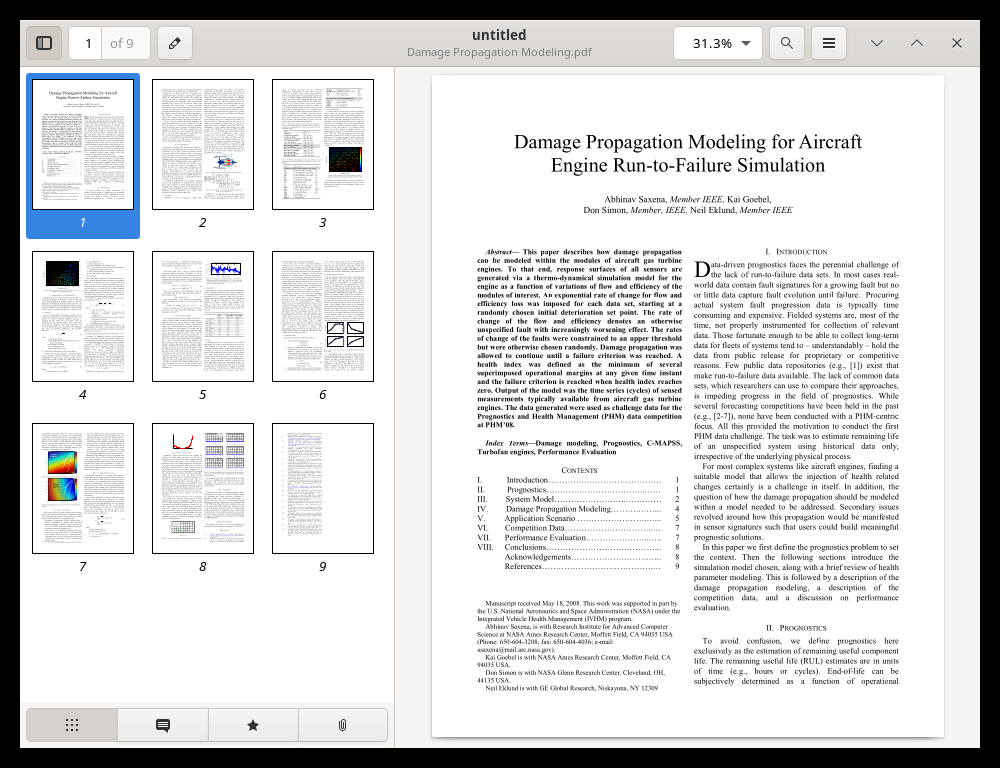
\includegraphics[width=0.55\textwidth]{images/data-source-01-paper.png}
  \caption{Makalah referensi dataset C-MAPSS (Saxena et al., PHM08)}
  \label{fig:paper}
\end{figure}

Empat sub-dataset tersedia dengan karakteristik berbeda, memungkinkan
evaluasi model pada tingkat kompleksitas yang bervariasi:

\begin{table}[H]
\centering\small
\caption{Karakteristik empat sub-dataset C-MAPSS}
\label{tab:dataset}
\begin{tabular}{lcccccc}
\toprule
Sub-dataset & Kondisi & Mode Kerusakan &
  \multicolumn{2}{c}{Jumlah Mesin} &
  \multicolumn{2}{c}{Jumlah Baris} \\
\cmidrule(lr){4-5}\cmidrule(lr){6-7}
& Operasi & & Train & Test & Train & Test \\
\midrule
FD001 & 1 & HPC         & 100 & 100 & 20.631 & 13.096 \\
FD002 & 6 & HPC         & 260 & 259 & 53.759 & 33.991 \\
FD003 & 1 & HPC + Fan   & 100 & 100 & 24.720 & 16.596 \\
FD004 & 6 & HPC + Fan   & 248 & 248 & 61.249 & 41.214 \\
\bottomrule
\end{tabular}
\end{table}

\subsection{Kolom dan Sensor}

Setiap baris data terdiri dari 26 kolom tanpa \textit{header}:

\begin{table}[H]
\centering\small
\caption{Deskripsi 26 kolom data C-MAPSS}
\label{tab:columns}
\begin{tabular}{lll}
\toprule
Kolom & Nama & Keterangan \\
\midrule
1   & \texttt{unit\_number}   & Nomor identitas mesin \\
2   & \texttt{time\_cycles}   & Siklus operasi (bertambah 1 tiap baris) \\
3--5 & \texttt{op\_setting\_1/2/3} & Pengaturan kondisi operasi \\
6--26 & sensor (21 buah) & Pembacaan sensor fisik mesin \\
\bottomrule
\end{tabular}
\end{table}

Konsep \textit{Remaining Useful Life} pada dataset ini bekerja sebagai berikut:
data \textit{train} mencatat siklus penuh hingga kegagalan sehingga RUL dapat
dihitung langsung ($\text{RUL} = t_{\max} - t_{\text{saat ini}}$). Data
\textit{test} dipotong sebelum kegagalan, dan file \texttt{RUL\_FDxxx.txt}
berisi RUL sebenarnya pada titik pemotongan sebagai kunci jawaban evaluasi.

\begin{figure}[H]
  \centering
  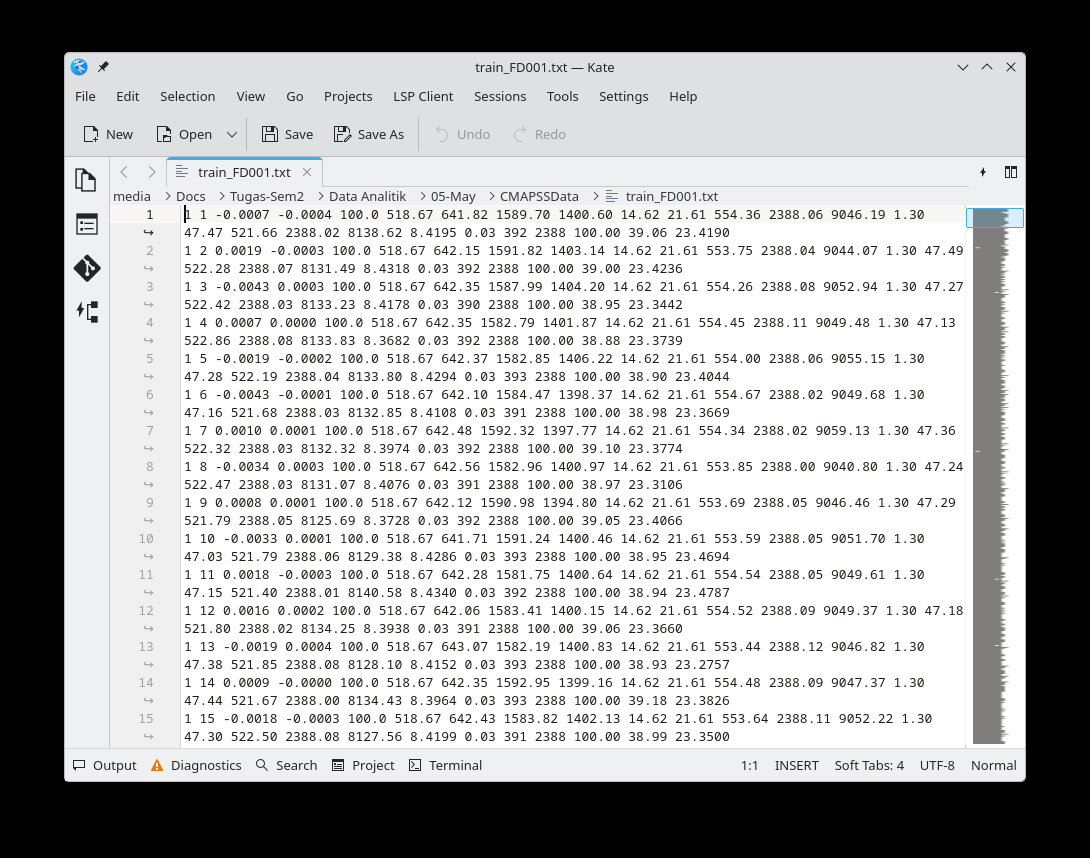
\includegraphics[width=0.75\textwidth]{images/data-source-02-data-train.png}
  \caption{Tampilan raw data \texttt{train\_FD001.txt} --- 26 kolom tanpa header}
  \label{fig:rawdata}
\end{figure}

\subsection{Struktur HDF5}

Seluruh data disimpan dalam format HDF5 menggunakan satu skrip konsolidasi
\texttt{build\_cmapss\_complete.py} yang membaca langsung dari file \texttt{.txt}
NASA tanpa file perantara. Satu file HDF5 per sub-dataset dihasilkan.

\begin{figure}[H]
  \centering
  \begin{subfigure}[b]{0.30\textwidth}
    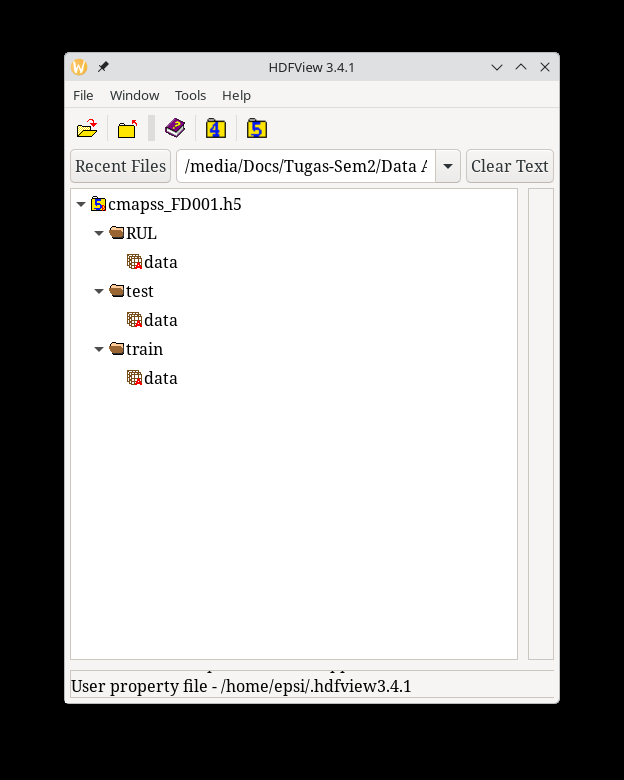
\includegraphics[width=\textwidth]{images/hdf5-01-vanilla-01-main.png}
    \caption{Vanilla HDF5}
  \end{subfigure}
  \hfill
  \begin{subfigure}[b]{0.30\textwidth}
    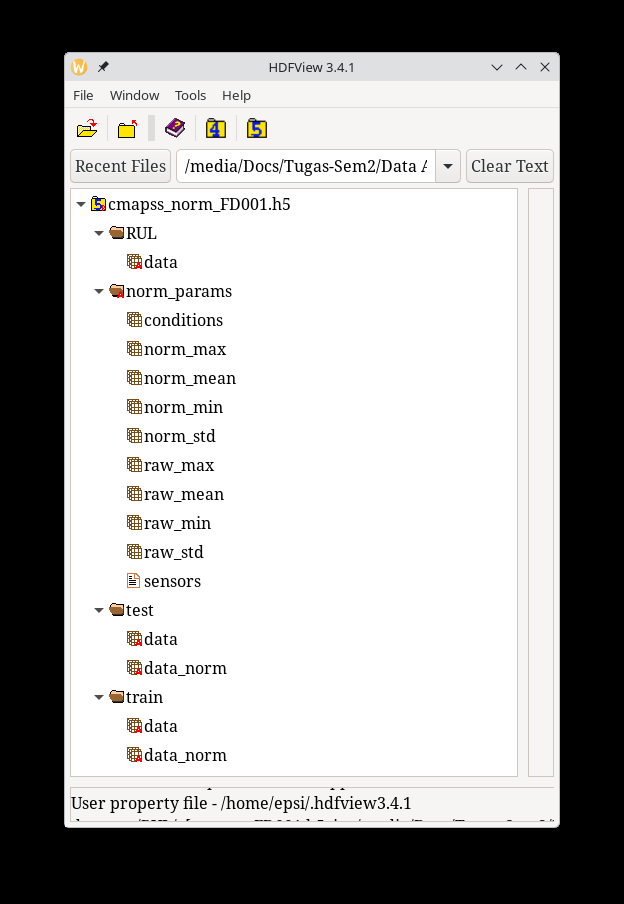
\includegraphics[width=\textwidth]{images/hdf5-03-normal-01-main.png}
    \caption{+ Normalisasi}
  \end{subfigure}
  \hfill
  \begin{subfigure}[b]{0.30\textwidth}
    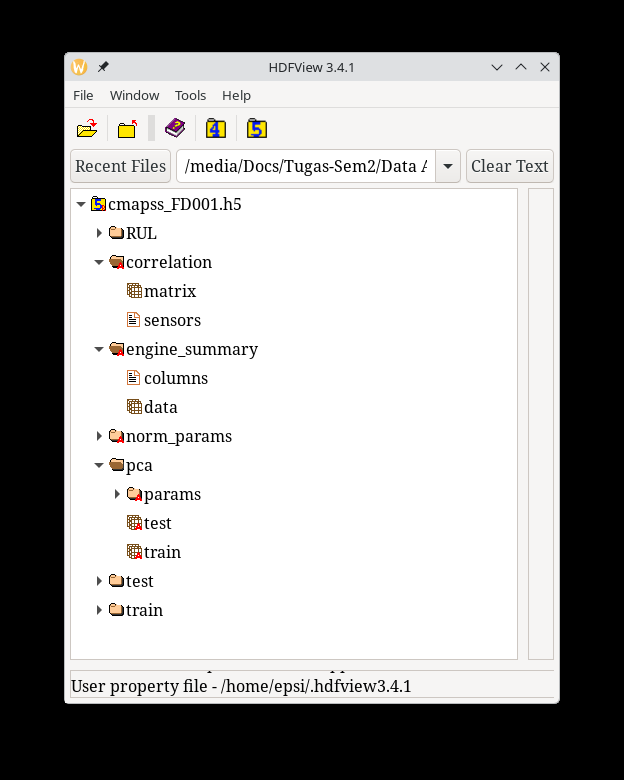
\includegraphics[width=\textwidth]{images/hdf5-05-pca-01-main.png}
    \caption{+ Korelasi + PCA}
  \end{subfigure}
  \caption{Evolusi struktur HDF5 dari vanilla hingga lengkap}
  \label{fig:hdf5_evolution}
\end{figure}

Struktur HDF5 final per file:

\begin{table}[H]
\centering\small
\caption{Struktur HDF5 lengkap \texttt{cmapss\_FDxxx.h5}}
\label{tab:hdf5}
\begin{tabular}{llp{6cm}}
\toprule
Path & Dimensi & Isi \\
\midrule
\texttt{/train/data}       & $(n, 32)$        & 26 kolom raw + 6 kolom komputasi \\
\texttt{/train/data\_norm} & $(n, n_s)$       & Sensor ternormalisasi \\
\texttt{/test/data}        & $(n, 29)$        & 26 raw + 3 kolom komputasi \\
\texttt{/test/data\_norm}  & $(n, n_s)$       & Sensor ternormalisasi (param train) \\
\texttt{/RUL/data}         & $(n_e, 4)$       & unit, rul, last\_cycle, total\_life\_est \\
\texttt{/norm\_params}     & $(n_c, n_s)$     & Parameter normalisasi per kondisi \\
\texttt{/correlation/matrix} & $(21, 21)$     & Matriks korelasi Pearson \\
\texttt{/engine\_summary/data} & $(n_e, 11)$  & Ringkasan per mesin train \\
\texttt{/pca/params}       & ---              & Eigenvectors dan varians \\
\texttt{/pca/train}        & $(n, 3+k)$       & Meta + skor PC (train) \\
\texttt{/pca/test}         & $(n, 3+k)$       & Meta + skor PC (test) \\
\bottomrule
\multicolumn{3}{l}{\small $n_s$: jumlah sensor; $n_e$: jumlah mesin; $n_c$: jumlah kondisi; $k$: jumlah komponen PCA}
\end{tabular}
\end{table}

% ══════════════════════════════════════════════════════════════════════════════
\section{Pembersihan Data}

\subsection{Identifikasi Sensor Tidak Informatif}

Lima metode statistik digunakan secara bersamaan untuk mengidentifikasi sensor
yang tidak membawa informasi degradasi:

\begin{enumerate}[noitemsep]
  \item \textbf{Standar Deviasi (std)} --- sensor dengan std $\approx 0$ bersifat konstan
  \item \textbf{Koefisien Variasi (CV)} --- $\text{CV} = \sigma/|\mu|$;
    nilai $< 0{,}001$ menunjukkan variasi yang tidak signifikan
  \item \textbf{Korelasi Pearson} dengan RUL --- hubungan linear; nilai $\approx 0$
    berarti tidak ada hubungan linear
  \item \textbf{Korelasi Spearman} dengan RUL --- hubungan monoton; lebih robust
    terhadap non-linearitas
  \item \textbf{Mutual Information} (MI) dengan RUL --- menangkap hubungan
    non-linear; nilai $\approx 0$ berarti tidak ada hubungan sama sekali
\end{enumerate}

\subsection{Tabel Statistik Sensor FD001}

\begin{table}[H]
\centering\small
\caption{Statistik lengkap sensor FD001 --- sensor dengan std $= 0$ ditandai ($\dagger$)}
\label{tab:sensor_stats}
\begin{tabular}{lrrrrrrl}
\toprule
Sensor & Mean & Std & CV & Pearson & Spearman & MI & Drop \\
\midrule
T2$^\dagger$        & 518.67 & 0.000 & 0.000 & NaN    & NaN    & 0.000 & \checkmark \\
T24          & 642.68 & 0.500 & 0.001 & $-$0.607 & $-$0.629 & 0.342 & \\
T30          & 1590.5 & 6.131 & 0.004 & $-$0.585 & $-$0.606 & 0.306 & \\
T50          & 1408.9 & 9.001 & 0.006 & $-$0.679 & $-$0.702 & 0.467 & \\
P2$^\dagger$        &  14.62 & 0.000 & 0.000 & NaN    & NaN    & 0.006 & \checkmark \\
P15          &  21.61 & 0.001 & 0.000 & $-$0.128 & $-$0.128 & 0.006 & \checkmark \\
P30          & 553.37 & 0.885 & 0.002 & $+$0.657 & $+$0.679 & 0.425 & \\
Nf           & 2388.1 & 0.071 & 0.000 & $-$0.564 & $-$0.574 & 0.258 & \\
Nc           & 9065.2 & 22.08 & 0.002 & $-$0.390 & $-$0.322 & 0.222 & \\
epr$^\dagger$       &   1.30 & 0.000 & 0.000 & NaN    & NaN    & 0.000 & \checkmark \\
Ps30         &  47.54 & 0.267 & 0.006 & $-$0.696 & $-$0.718 & 0.507 & \\
phi          & 521.41 & 0.738 & 0.001 & $+$0.672 & $+$0.693 & 0.442 & \\
NRf          & 2388.1 & 0.072 & 0.000 & $-$0.563 & $-$0.573 & 0.262 & \\
NRc          & 8143.8 & 19.08 & 0.002 & $-$0.307 & $-$0.202 & 0.225 & \\
BPR          &   8.44 & 0.038 & 0.004 & $-$0.643 & $-$0.666 & 0.390 & \\
farB$^\dagger$      &   0.03 & 0.000 & 0.000 & NaN    & NaN    & 0.000 & \checkmark \\
htBleed      & 393.21 & 1.549 & 0.004 & $-$0.606 & $-$0.629 & 0.328 & \\
Nf\_dmd$^\dagger$   & 2388.0 & 0.000 & 0.000 & NaN    & NaN    & 0.000 & \checkmark \\
PCNfR\_dmd$^\dagger$& 100.00 & 0.000 & 0.000 & NaN    & NaN    & 0.000 & \checkmark \\
W31          &  38.82 & 0.181 & 0.005 & $+$0.629 & $+$0.653 & 0.367 & \\
W32          &  23.29 & 0.108 & 0.005 & $+$0.636 & $+$0.657 & 0.380 & \\
\bottomrule
\multicolumn{8}{l}{\small $^\dagger$ Konstan (std $= 0$); Pearson/Spearman tidak terdefinisi (NaN); dieliminasi}
\end{tabular}
\end{table}

Untuk sub-dataset lain, analisis serupa dilakukan. Hasilnya:
FD002 dan FD004 tidak mengeliminasi sensor apapun karena variasi antar
6 kondisi operasi membuat semua sensor bervariasi.
FD003 mengeliminasi 5 sensor yang sama dengan FD001, kecuali \texttt{epr}
yang memiliki std $= 0{,}0035$ (kecil namun tidak nol) akibat mode kerusakan
HPC+Fan.

\subsection{Hasil Eliminasi per Sub-dataset}

\begin{table}[H]
\centering\small
\caption{Sensor yang dieliminasi per sub-dataset}
\label{tab:drop}
\begin{tabular}{lcp{8cm}}
\toprule
Sub-dataset & Dihapus & Sensor \\
\midrule
FD001 & 6 & T2, P2, epr, farB, Nf\_dmd, PCNfR\_dmd \\
FD002 & 0 & (tidak ada --- semua sensor bervariasi antar 6 kondisi) \\
FD003 & 5 & T2, P2, farB, Nf\_dmd, PCNfR\_dmd \\
FD004 & 0 & (tidak ada) \\
\bottomrule
\end{tabular}
\end{table}

% ══════════════════════════════════════════════════════════════════════════════
\section{Normalisasi}

\subsection{Formula Z-Score}

Normalisasi \textit{z-score} mentransformasi setiap pembacaan sensor menjadi
jumlah standar deviasi dari nilai referensi:

\begin{equation}
  z = \frac{x - \mu_c}{\sigma_c}
  \label{eq:zscore}
\end{equation}

di mana $\mu_c$ dan $\sigma_c$ adalah mean dan standar deviasi untuk
kondisi operasi $c$.

\subsection{Mengapa Hanya Siklus Sehat}

Parameter $\mu_c$ dan $\sigma_c$ dihitung hanya dari siklus dengan
RUL\_raw $\geq 125$ (\textit{healthy cycles}).
Alasannya: jika parameter dihitung dari seluruh siklus termasuk yang
terdegradasi, maka nilai $z = 0$ tidak lagi merepresentasikan kondisi sehat
--- melainkan rata-rata dari sehat hingga menjelang gagal. Akibatnya, sinyal
degradasi menjadi kabur.

Dengan menggunakan siklus sehat sebagai referensi:
\begin{itemize}[noitemsep]
  \item Siklus sehat $\rightarrow$ $z \approx 0$
  \item Siklus terdegradasi $\rightarrow$ $z$ menyimpang dari 0
  \item Penyimpangan dari 0 = sinyal degradasi yang dapat dipelajari model
\end{itemize}

\subsection{Mengapa Per Kondisi, Bukan Global}

Pada FD002 dan FD004 terdapat 6 kondisi operasi (ketinggian dan kecepatan
penerbangan berbeda). Sensor seperti T2 (\textit{fan inlet temperature}) memiliki
nilai $\approx 518$\,R pada kondisi 1 namun $\approx 445$\,R pada kondisi lain
--- perbedaan 73\,R ini bukan akibat degradasi, melainkan perbedaan kondisi
operasi.

Normalisasi global akan menganggap selisih ini sebagai penyimpangan
dan mengaburkan sinyal degradasi yang sebenarnya. Normalisasi per kondisi
menghilangkan efek kondisi operasi terlebih dahulu, menyisakan hanya sinyal
degradasi.

\subsection{Penerapan ke Data Test}

Data \textit{test} dinormalisasi menggunakan parameter yang dihitung dari
data \textit{train}:

\begin{equation}
  z_{\text{test}} = \frac{x_{\text{test}} - \mu_{c,\,\text{train}}}{\sigma_{c,\,\text{train}}}
\end{equation}

Menggunakan parameter \textit{test} sendiri (\textit{data leakage}) adalah keliru
karena pada kondisi \textit{deployment} nyata, distribusi data masa depan tidak
diketahui. Parameter harus dibekukan dari data \textit{train}.

% ══════════════════════════════════════════════════════════════════════════════
\section{Seleksi Fitur}

\subsection{Korelasi Pearson}

Matriks korelasi Pearson dihitung dari \texttt{train\_normalized} untuk
seluruh 21 sensor. Sensor konstan menghasilkan baris dan kolom \texttt{NaN}.

\begin{figure}[H]
  \centering
  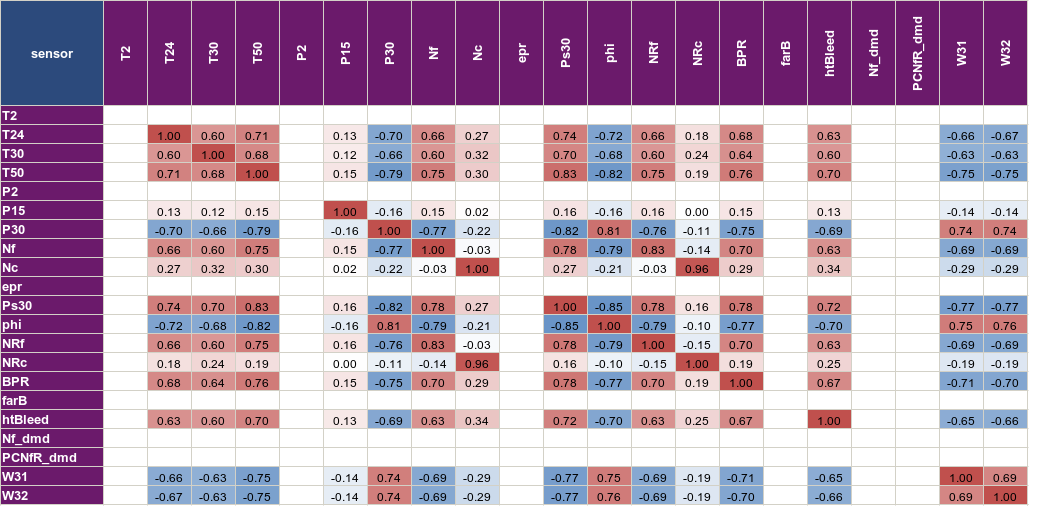
\includegraphics[width=0.80\textwidth]{images/spreadsheet-05-correlation-05-correlations.png}
  \caption{Matriks korelasi Pearson antar sensor (FD001) di spreadsheet v5}
  \label{fig:corr}
\end{figure}

Dari matriks korelasi, teridentifikasi:
\begin{itemize}[noitemsep]
  \item \textbf{Sensor kuat negatif vs RUL}: Ps30 ($-0{,}70$), T50 ($-0{,}68$),
    phi ($+0{,}67$) --- sensor ini paling relevan untuk prediksi
  \item \textbf{Redundansi}: Nf--NRf ($r = 0{,}83$), Nc--NRc ($r = 0{,}96$) ---
    pasangan ini membawa informasi yang hampir sama, motivasi utama PCA
\end{itemize}

\subsection{Principal Component Analysis (PCA)}

\subsubsection{Varians yang Dijelaskan}

PCA diterapkan pada \texttt{train\_normalized}. Komponen diurutkan dari yang
menjelaskan varians terbesar. Tabel \ref{tab:pca_variance} menunjukkan
varians individual dan kumulatif.

\begin{table}[H]
\centering\small
\caption{Varians PCA per sub-dataset (8 komponen pertama)}
\label{tab:pca_variance}
\begin{tabular}{lrrrrrrrr}
\toprule
Sub-dataset & PC1 & PC2 & PC3 & PC4 & PC5 & PC6 & PC7 & PC8 \\
\midrule
FD001 & 52,4\% & 30,5\% & 2,0\% & 1,8\% & 1,7\% & 1,6\% & 1,6\% & 1,4\% \\
FD002 & 41,6\% & 19,5\% & 8,4\% & 5,3\% & 4,8\% & 2,3\% & 2,1\% & 1,9\% \\
FD003 & 60,2\% & 20,4\% & 7,2\% & 3,9\% & 1,7\% & 1,1\% & 1,0\% & 0,9\% \\
FD004 & 48,4\% & 20,9\% & 8,1\% & 4,3\% & 2,7\% & 2,4\% & 2,0\% & 1,7\% \\
\bottomrule
\end{tabular}
\end{table}

Pada FD001 terdapat \textit{scree cliff} setelah PC2: PC1 = 52,4\% dan
PC2 = 30,5\%, kemudian PC3 hanya 2,0\%. Ini menunjukkan dua komponen pertama
mendominasi informasi.

\subsubsection{Pemilihan Jumlah Komponen --- Opsi B}

Kriteria pemilihan: pertahankan komponen dengan varians individual $\geq 5\%$.
Alasan: komponen di bawah 5\% sebagian besar merupakan \textit{noise} sisa
setelah informasi utama terekstrak.

\begin{table}[H]
\centering\small
\caption{Jumlah komponen PCA yang dipertahankan (Opsi B, varians $\geq 5\%$)}
\label{tab:pca_kept}
\begin{tabular}{lcccc}
\toprule
Sub-dataset & Sensor & Komponen & Varians Kumulatif & Komponen yang Dipertahankan \\
\midrule
FD001 & 15 & 2 & 82,9\% & PC1, PC2 \\
FD002 & 21 & 4 & 74,8\% & PC1, PC2, PC3, PC4 \\
FD003 & 16 & 3 & 87,8\% & PC1, PC2, PC3 \\
FD004 & 21 & 3 & 77,5\% & PC1, PC2, PC3 \\
\bottomrule
\end{tabular}
\end{table}

\subsubsection{Interpretasi Eigenvectors}

\begin{figure}[H]
  \centering
  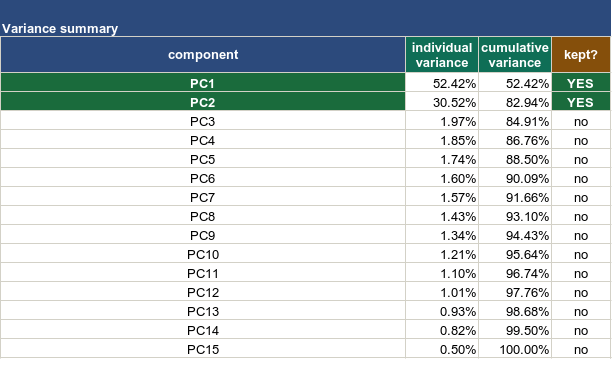
\includegraphics[width=0.80\textwidth]{images/spreadsheet-06-pca-11a-pca-params.png}
  \caption{Tabel varians dan matriks \textit{eigenvectors} pada spreadsheet v6 (FD002)}
  \label{fig:pca_params}
\end{figure}

Interpretasi fisik komponen FD002:
\begin{itemize}[noitemsep]
  \item \textbf{PC1} (41,6\%): didominasi Nf, NRf, Nc, NRc ---
    merepresentasikan \textit{overall engine speed state}
  \item \textbf{PC2} (19,5\%): kontras NRc/Nc positif vs Ps30/BPR/T50 negatif ---
    merepresentasikan \textit{compressor loading condition}
  \item \textbf{PC3} (8,4\%): epr dengan \textit{loading} $= 0{,}940$ ---
    hampir seluruhnya merupakan \textit{engine pressure ratio};
    terisolasi karena bervariasi berbeda dari sensor lain antar kondisi operasi
  \item \textbf{PC4} (5,3\%): farB positif vs Nc/NRc negatif ---
    merepresentasikan \textit{fuel combustion efficiency}
\end{itemize}

% ══════════════════════════════════════════════════════════════════════════════
\section{Pipeline Spreadsheet}

Paralel dengan pipeline HDF5, seluruh data dan analisis juga didokumentasikan
dalam format spreadsheet LibreOffice Calc (kompatibel Excel) melalui enam
versi iteratif.

\begin{figure}[H]
  \centering
  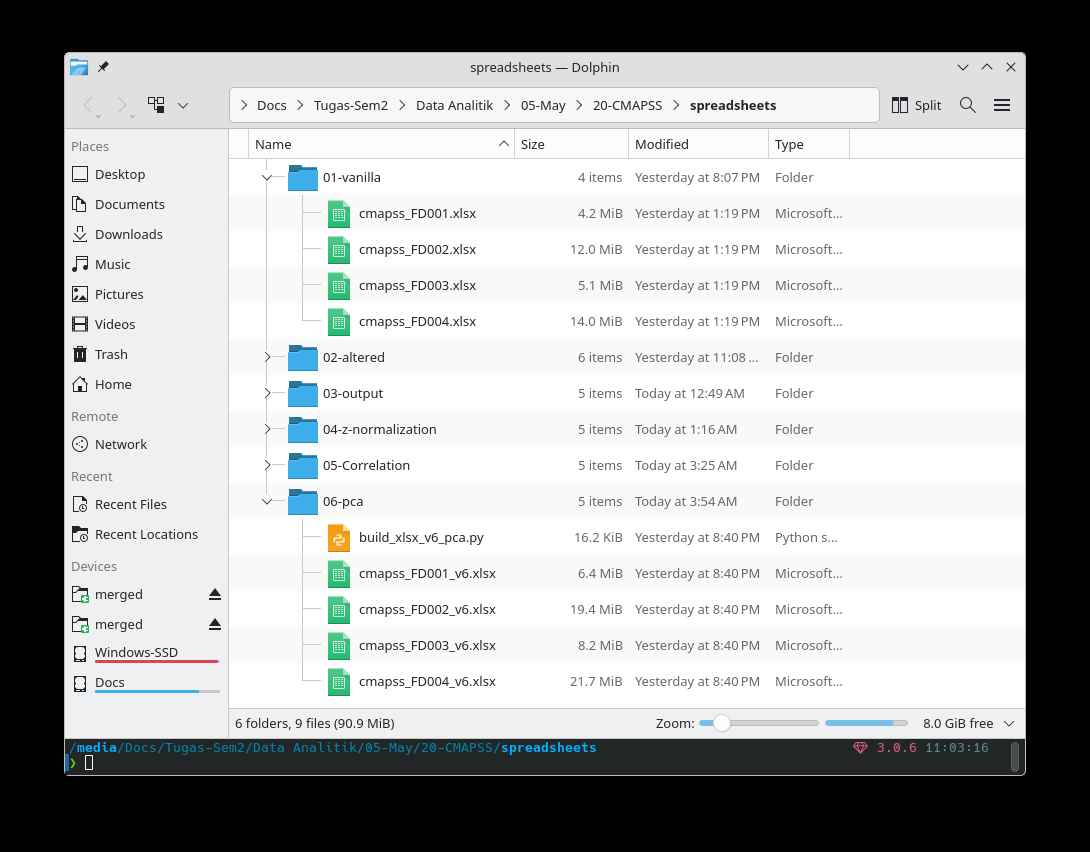
\includegraphics[width=0.75\textwidth]{images/workbook-00-working-directories.png}
  \caption{Struktur direktori spreadsheet --- enam versi iteratif (v1--v6)}
  \label{fig:workbook_dir}
\end{figure}

\begin{table}[H]
\centering\small
\caption{Evolusi spreadsheet v1--v6 dan sheet yang ditambahkan}
\label{tab:spreadsheet}
\begin{tabular}{llp{9cm}}
\toprule
Versi & Sheet Baru & Isi \\
\midrule
v1 & \texttt{train} & Data raw 26 kolom \\
v2 & \texttt{test}, \texttt{RUL} & Data test + RUL dengan last\_cycle dan total\_life\_est \\
v3 & --- & Penambahan kolom komputasi (condition\_id, dT, RUL\_raw, dll.) \\
v4 & \texttt{train\_normalized} & Sensor ternormalisasi (z-score per kondisi) \\
v5 & \texttt{test\_normalized}, \texttt{stats}, \texttt{correlation}, \texttt{engine\_summary}
   & Normalisasi test, statistik per sensor, matriks korelasi, ringkasan mesin \\
v6 & \texttt{pca\_params}, \texttt{pca\_train}, \texttt{pca\_test}
   & Parameter PCA (eigenvectors, varians), skor PCA train dan test \\
\bottomrule
\end{tabular}
\end{table}

\begin{figure}[H]
  \centering
  \begin{subfigure}[b]{0.48\textwidth}
    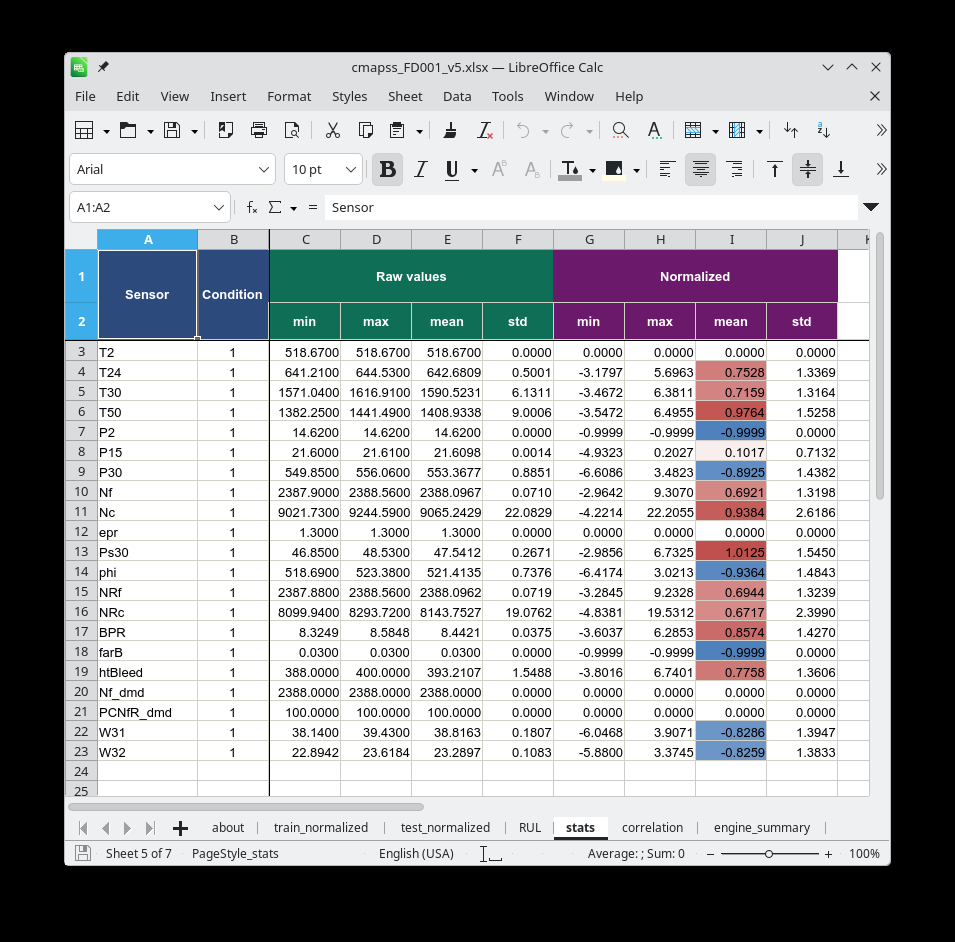
\includegraphics[width=\textwidth]{images/workbook-05-correlation-04-statistics.png}
    \caption{Sheet \texttt{stats} (v5) --- statistik raw dan ternormalisasi}
  \end{subfigure}
  \hfill
  \begin{subfigure}[b]{0.48\textwidth}
    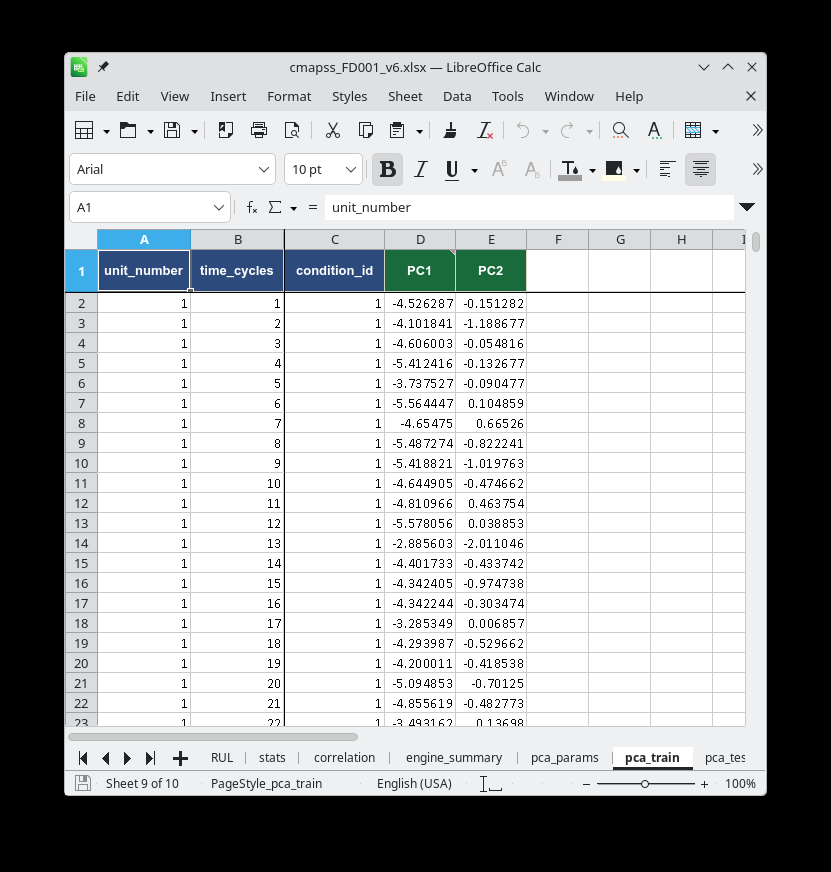
\includegraphics[width=\textwidth]{images/workbook-06-pca-12-pca-train.png}
    \caption{Sheet \texttt{pca\_train} (v6) --- skor PC per siklus}
  \end{subfigure}
  \caption{Contoh sheet pada spreadsheet v5 dan v6}
  \label{fig:spreadsheet_sheets}
\end{figure}

% ══════════════════════════════════════════════════════════════════════════════
\section{Model Artificial Neural Network}

\subsection{Arsitektur MLP}

Model \textit{Multilayer Perceptron} (MLP) dengan arsitektur tiga lapisan:

\begin{equation}
  \text{input} \xrightarrow{W_1} 64 \xrightarrow{\text{ReLU}}
  \xrightarrow{W_2} 32 \xrightarrow{\text{ReLU}}
  \xrightarrow{W_3} 1
\end{equation}

\begin{table}[H]
\centering\small
\caption{Konfigurasi pelatihan model ANN}
\label{tab:ann_config}
\begin{tabular}{ll}
\toprule
Parameter & Nilai \\
\midrule
Arsitektur    & input $\to$ 64 $\to$ 32 $\to$ 1 \\
Aktivasi      & ReLU (tersembunyi), Linear (output) \\
\textit{Loss} & MSE (\textit{Mean Squared Error}) \\
Optimizer     & Adam, $\text{lr} = 10^{-3}$ \\
Epoch         & 500 \\
Batch size    & 512 \\
\bottomrule
\end{tabular}
\end{table}

\subsection{Target: RUL Capped}

Target pelatihan menggunakan \texttt{RUL\_capped} dengan cap $= 125$ siklus,
bukan \texttt{RUL\_raw}. Alasannya: pada siklus awal ketika mesin masih sehat,
pembacaan sensor hampir identik meskipun nilai RUL\_raw berbeda (mis.\ 300 vs
250 siklus). Model tidak dapat membedakan keduanya dari sensor. Cap 125
menyederhanakan target: semua siklus sehat diperlakukan setara, dan model
difokuskan pada fase degradasi di mana sinyal sensor benar-benar bervariasi.

\subsection{Desain Eksperimen Benchmark}

Benchmark dirancang sebagai eksperimen 2-faktor:

\begin{itemize}[noitemsep]
  \item \textbf{Faktor 1} --- Sub-dataset: FD001, FD002, FD003, FD004
  \item \textbf{Faktor 2} --- Tipe input: PCA (skor PC) vs NORM (semua sensor ternormalisasi)
  \item \textbf{Total}: $4 \times 2 = 8$ model
\end{itemize}

\begin{figure}[H]
  \centering
  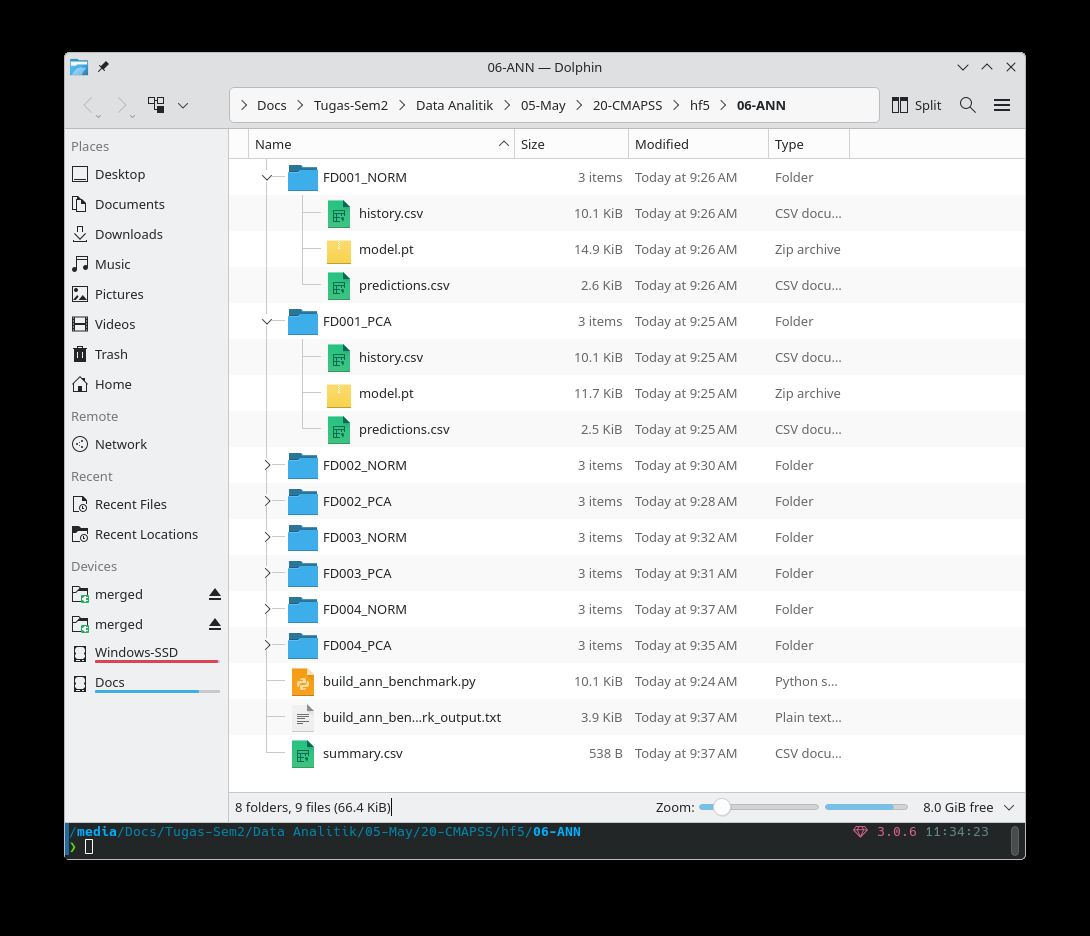
\includegraphics[width=0.75\textwidth]{images/ann-06-working-directories.png}
  \caption{Struktur direktori hasil benchmark --- 8 subfolder + \texttt{summary.csv}}
  \label{fig:ann_dir}
\end{figure}

\subsection{Hasil Benchmark}

\begin{table}[H]
\centering\small
\caption{Hasil benchmark 8 model (500 epoch, batch 512)}
\label{tab:benchmark}
\begin{tabular}{llcrrr}
\toprule
Sub-dataset & Input & Dim & RMSE & MAE & NASA Score \\
\midrule
FD001 & \textbf{PCA}  & 2  & \textbf{17,80} & \textbf{12,55} & \textbf{815} \\
FD001 & NORM & 15 & 18,21 & 13,52 & 929 \\
\midrule
FD002 & \textbf{PCA}  & 4  & \textbf{29,30} & \textbf{20,52} & 14.423 \\
FD002 & NORM & 21 & 29,45 & 20,73 & \textbf{12.990} \\
\midrule
FD003 & PCA  & 3  & 21,87 & 16,17 & 2.650 \\
FD003 & \textbf{NORM} & 16 & \textbf{20,16} & \textbf{15,28} & \textbf{1.783} \\
\midrule
FD004 & PCA  & 3  & 30,59 & 23,28 & 9.267 \\
FD004 & \textbf{NORM} & 21 & \textbf{29,68} & \textbf{22,38} & \textbf{7.157} \\
\bottomrule
\end{tabular}
\end{table}

\begin{figure}[H]
  \centering
  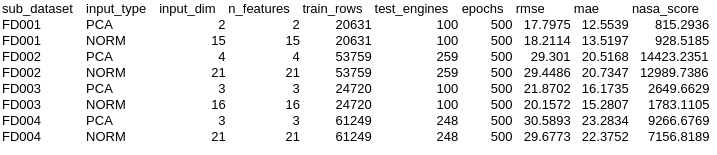
\includegraphics[width=0.72\textwidth]{images/ann-06-00-summary.png}
  \caption{File \texttt{summary.csv} hasil benchmark di LibreOffice Calc}
  \label{fig:summary}
\end{figure}

\subsection{Analisis Hasil}

\textbf{Pengaruh Faktor 1 --- Kompleksitas Sub-dataset:}

\begin{table}[H]
\centering\small
\caption{RMSE rata-rata per sub-dataset (rerata PCA dan NORM)}
\label{tab:complexity}
\begin{tabular}{lcccc}
\toprule
 & FD001 & FD003 & FD002 & FD004 \\
\cmidrule(lr){2-3}\cmidrule(lr){4-5}
Kondisi operasi & \multicolumn{2}{c}{1} & \multicolumn{2}{c}{6} \\
Mode kerusakan  & HPC & HPC+Fan & HPC & HPC+Fan \\
RMSE rata-rata  & 18,0 & 21,0 & 29,4 & 30,1 \\
\bottomrule
\end{tabular}
\end{table}

Sub-dataset dengan 6 kondisi operasi menghasilkan RMSE $\approx 60\%$ lebih
tinggi dibandingkan 1 kondisi. Ini adalah faktor dominan yang melebihi
pengaruh tipe input.

\textbf{Pengaruh Faktor 2 --- Tipe Input:}

Terdapat interaksi antara kedua faktor: PCA lebih baik pada dataset
\textit{sederhana} (FD001, FD002 berdasarkan RMSE), sedangkan NORM lebih baik
pada dataset \textit{kompleks} (FD003, FD004). Hal ini konsisten dengan teori:
kompresi PCA membuang 17\% varians yang justru relevan ketika terdapat
kompleksitas lebih tinggi (dua mode kerusakan atau 6 kondisi operasi).

\textbf{NASA Score FD002 yang Anomali:}

NASA score FD002 (14.423) jauh lebih tinggi dibandingkan FD001 (815).
NASA score menggunakan penalti eksponensial asimetris: prediksi \textit{late}
(overestimasi RUL) dihukum lebih berat ($e^{d/10}$) dibandingkan prediksi
\textit{early} ($e^{d/13}$). Pada FD002 dengan 6 kondisi operasi yang
kompleks, model cenderung overestimasi RUL pada banyak mesin,
mengakibatkan akumulasi penalti eksponensial yang tinggi.

\subsection{Loss Curve}

\begin{figure}[H]
  \centering
  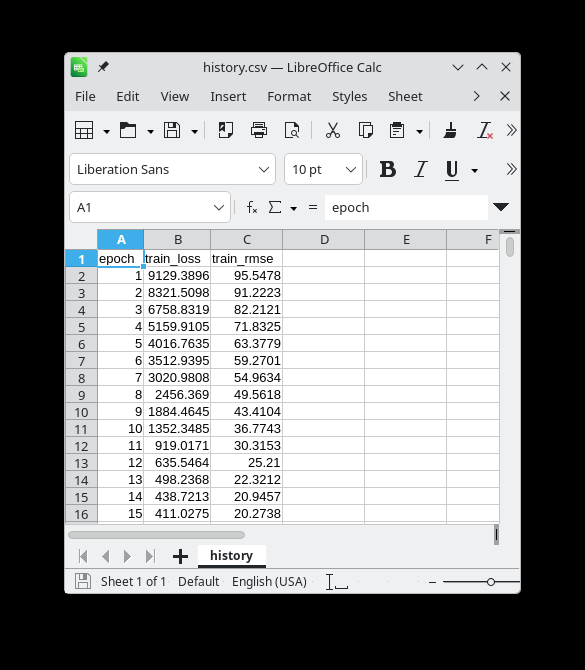
\includegraphics[width=0.72\textwidth]{images/ann-06-01-norm-history.png}
  \caption{\textit{Training loss} (RMSE) per epoch --- FD001 NORM}
  \label{fig:loss_curve}
\end{figure}

Kurva \textit{loss} FD001 menunjukkan konvergensi yang hampir penuh setelah
$\approx 200$ epoch; epoch 200--500 hanya menghasilkan penurunan kecil
(17,77 $\to$ 17,30). Model PCA konvergen lebih cepat karena dimensi input
lebih kecil (2 vs 15 fitur).

% ══════════════════════════════════════════════════════════════════════════════
\section{Analisis Garson}

\subsection{Algoritma}

Algoritma Garson \cite{garson1991} menghitung kepentingan relatif setiap fitur
input berdasarkan bobot jaringan yang telah dilatih. Untuk arsitektur dua
lapisan tersembunyi dengan matriks bobot $W_1$, $W_2$, $W_3$:

\begin{align}
  q_1[i,j] &= \frac{|W_1[j,i]|}{\sum_k |W_1[j,k]|} &
  q_2[j,m] &= \frac{|W_2[m,j]|}{\sum_k |W_2[m,k]|} \\[4pt]
  r[i,m]   &= \sum_j q_1[i,j] \cdot q_2[j,m] &
  s[i]     &= \sum_m r[i,m] \cdot |W_3[m]| \\[4pt]
  \text{importance}[i] &= \frac{s[i]}{\sum_k s[k]}
\end{align}

Hasilnya adalah satu skor kepentingan per fitur input, dengan total 100\%.

\subsection{Hasil per Model}

\begin{figure}[H]
  \centering
  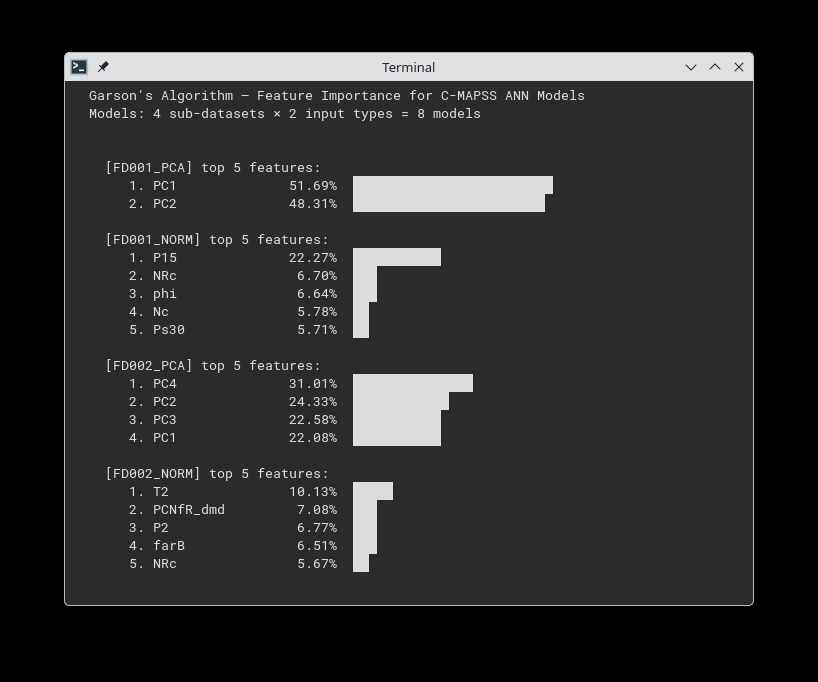
\includegraphics[width=0.72\textwidth]{images/python-09-garson-term-01.png}
  \caption{Output terminal algoritma Garson --- top 5 fitur FD001 dan FD002}
  \label{fig:garson_term}
\end{figure}

\begin{table}[H]
\centering\small
\caption{Lima fitur terpenting per model (algoritma Garson)}
\label{tab:garson}
\begin{tabular}{llp{9.5cm}}
\toprule
Model & Fitur \#1 & Top 5 Fitur (kepentingan \%) \\
\midrule
FD001\_PCA  & PC1 (51,7\%)
  & PC1 51,7\% --- PC2 48,3\% \\
FD001\_NORM & P15 (22,3\%)
  & P15 22,3\% --- NRc 6,7\% --- phi 6,6\% --- Nc 5,8\% --- Ps30 5,7\% \\
FD002\_PCA  & PC4 (31,0\%)
  & PC4 31,0\% --- PC2 24,3\% --- PC3 22,6\% --- PC1 22,1\% \\
FD002\_NORM & T2 (10,1\%)
  & T2 10,1\% --- PCNfR\_dmd 7,1\% --- P2 6,8\% --- farB 6,5\% --- NRc 5,7\% \\
FD003\_PCA  & PC2 (37,9\%)
  & PC2 37,9\% --- PC3 35,7\% --- PC1 26,5\% \\
FD003\_NORM & P15 (14,7\%)
  & P15 14,7\% --- epr 8,0\% --- phi 6,8\% --- P30 6,4\% --- NRc 6,3\% \\
FD004\_PCA  & PC2 (42,3\%)
  & PC2 42,3\% --- PC3 31,8\% --- PC1 26,0\% \\
FD004\_NORM & T2 (9,9\%)
  & T2 9,9\% --- P2 9,3\% --- P15 8,4\% --- Ps30 5,5\% --- phi 5,2\% \\
\bottomrule
\end{tabular}
\end{table}

\subsection{Perbandingan Tiga Metode Seleksi Fitur}

\begin{table}[H]
\centering\small
\caption{Perbandingan kepentingan sensor berdasarkan tiga metode (FD001)}
\label{tab:three_method}
\begin{tabular}{lcccl}
\toprule
Sensor & Pearson & PCA Loading & Garson & Interpretasi \\
\midrule
Ps30  & $-0{,}70$ & tinggi   & sedang  & Konsisten --- penting secara linear \\
T50   & $-0{,}68$ & tinggi   & sedang  & Konsisten --- penting secara linear \\
P30   & $+0{,}66$ & tinggi   & sedang  & Konsisten --- penting secara linear \\
\textbf{P15}
      & $-0{,}13$ & rendah   & \textbf{tinggi} &
        Perbedaan --- ANN menemukan sinyal non-linear \\
NRf   & $-0{,}56$ & sedang   & rendah  & Sebagian konsisten \\
\midrule
\multicolumn{5}{l}{\small\textit{Metode yang digunakan:}
  Pearson = korelasi linear dengan RUL;
  PCA = kontribusi variansi;
  Garson = kepentingan dalam bobot ANN} \\
\bottomrule
\end{tabular}
\end{table}

Temuan utama dari perbandingan tiga metode:

\begin{enumerate}[noitemsep]
  \item \textbf{P15} memiliki korelasi Pearson rendah ($-0{,}13$) dan kontribusi
    PCA rendah, namun Garson menetapkannya sebagai fitur terpenting (22,3\%) pada
    FD001\_NORM. Ini mengindikasikan ANN mengeksploitasi hubungan non-linear
    yang tidak terdeteksi oleh Pearson dan PCA.

  \item \textbf{FD002\_NORM}: T2, P2, PCNfR\_dmd, farB --- sensor yang dieliminasi
    dari FD001 karena std $= 0$ --- muncul sebagai fitur terpenting di FD002.
    Hal ini mengkonfirmasi eliminasi sensor harus dilakukan \textit{per sub-dataset},
    bukan secara universal.

  \item \textbf{Konsistensi Ps30 dan T50}: keduanya penting menurut ketiga metode,
    menjadikannya kandidat fitur paling andal untuk prediksi RUL secara umum.
\end{enumerate}

% ══════════════════════════════════════════════════════════════════════════════
\section{Keterbatasan dan Pengembangan}

\subsection{Keterbatasan}

\begin{enumerate}[noitemsep]
  \item \textbf{Arsitektur MLP sederhana}: model feedforward tidak memanfaatkan
    dependensi temporal antar siklus. Setiap siklus diperlakukan independen,
    padahal degradasi adalah proses sekuensial.
  \item \textbf{Dataset simulasi}: C-MAPSS adalah data simulasi, bukan data
    mesin nyata. Pola degradasi pada mesin nyata mungkin lebih kompleks dan
    tidak sebersih data simulasi.
  \item \textbf{Tanpa regularisasi}: model tidak menggunakan \textit{dropout}
    atau regularisasi lain. Gap antara \textit{train RMSE} (17,3) dan
    \textit{test RMSE} (18,2) pada FD001 mengindikasikan \textit{overfitting}
    ringan.
  \item \textbf{Garson untuk dua lapisan tersembunyi}: algoritma Garson
    orisinal dirancang untuk satu lapisan tersembunyi. Ekstensi ke dua
    lapisan yang digunakan di sini kurang didukung literatur dibandingkan
    versi satu lapisan.
\end{enumerate}

\subsection{Pengembangan yang Memungkinkan}

\begin{enumerate}[noitemsep]
  \item \textbf{LSTM / GRU}: memanfaatkan urutan temporal siklus untuk
    prediksi yang lebih akurat
  \item \textbf{Dropout regularisasi}: mengurangi \textit{overfitting} pada
    dataset dengan sensor penuh (NORM)
  \item \textbf{Normalisasi per kondisi lebih ketat}: menggunakan
    \textit{condition subtraction} sebelum PCA untuk dataset 6 kondisi
\end{enumerate}

% ══════════════════════════════════════════════════════════════════════════════
\section{Kesimpulan}

Pipeline analitik lengkap untuk prediksi RUL mesin turbofan C-MAPSS telah
berhasil diimplementasikan. Temuan utama:

\begin{enumerate}[noitemsep]
  \item \textbf{Kompleksitas kondisi operasi adalah faktor dominan}.
    Sub-dataset 6 kondisi (FD002, FD004) menghasilkan RMSE $\approx 60\%$
    lebih tinggi dari sub-dataset 1 kondisi (FD001, FD003),
    terlepas dari tipe input yang digunakan.

  \item \textbf{Tipe input optimal bergantung pada kompleksitas}.
    PCA lebih baik untuk dataset sederhana (1 kondisi); sensor ternormalisasi
    penuh lebih baik untuk dataset kompleks (2 mode kerusakan atau 6 kondisi).

  \item \textbf{Algoritma Garson mengungkap sinyal non-linear}.
    Sensor P15 --- yang memiliki korelasi Pearson rendah dan kontribusi PCA
    rendah --- terbukti menjadi fitur terpenting menurut Garson pada
    FD001\_NORM, menunjukkan ANN mampu mengeksploitasi hubungan non-linear.

  \item \textbf{Eliminasi sensor harus per sub-dataset}.
    Sensor konstan di FD001 (T2, P2) menjadi fitur terpenting di FD002
    karena variasi antar kondisi operasi mengandung informasi degradasi.
\end{enumerate}

% ── References ────────────────────────────────────────────────────────────────
\begin{thebibliography}{9}
\bibitem{saxena2008}
  A. Saxena, K. Goebel, D. Simon, N. Eklund,
  ``Damage Propagation Modeling for Aircraft Engine Run-to-Failure Simulation,''
  \textit{Proc.\ 1st Int.\ Conf.\ Prognostics and Health Management (PHM08)},
  Denver, CO, 2008.

\bibitem{garson1991}
  G.D. Garson,
  ``Interpreting Neural Network Connection Weights,''
  \textit{AI Expert}, vol.~6, no.~4, pp.~46--51, 1991.
\end{thebibliography}

\end{document}
